%%%%%%%%%%%%%%%%%%%%%%%%%%%%%%%%%%%%%%%%%
% Beamer Presentation
% LaTeX Template
% Version 1.0 (10/11/12)
%
% This template has been downloaded from:
% http://www.LaTeXTemplates.com
%
% License:
% CC BY-NC-SA 3.0 (http://creativecommons.org/licenses/by-nc-sa/3.0/)
%
%%%%%%%%%%%%%%%%%%%%%%%%%%%%%%%%%%%%%%%%%

%----------------------------------------------------------------------------------------
%	PACKAGES AND THEMES
%----------------------------------------------------------------------------------------

\documentclass{beamer}

\mode<presentation> {

% The Beamer class comes with a number of default slide themes
% which change the colors and layouts of slides. Below this is a list
% of all the themes, uncomment each in turn to see what they look like.

%\usetheme{default}
%\usetheme{AnnArbor}
%\usetheme{Antibes}
%\usetheme{Bergen}
%\usetheme{Berkeley}
%\usetheme{Berlin}
%\usetheme{Boadilla}
%\usetheme{CambridgeUS}
%\usetheme{Copenhagen}
%\usetheme{Darmstadt}
%\usetheme{Dresden}
%\usetheme{Frankfurt}
%\usetheme{Goettingen}
%\usetheme{Hannover}
\usetheme{Ilmenau}
%\usetheme{JuanLesPins}
%\usetheme{Luebeck}
%\usetheme{Madrid}
%\usetheme{Malmoe}
%\usetheme{Marburg}
%\usetheme{Montpellier}
%\usetheme{PaloAlto}
%\usetheme{Pittsburgh}
%\usetheme{Rochester}
%\usetheme{Singapore}
%\usetheme{Szeged}
%\usetheme{Warsaw}
%\usetheme{Feather}

% As well as themes, the Beamer class has a number of color themes
% for any slide theme. Uncomment each of these in turn to see how it
% changes the colors of your current slide theme.

%\usecolortheme{albatross}
%\usecolortheme{beaver}
%\usecolortheme{beetle}
%\usecolortheme{crane}
%\usecolortheme{dolphin}
%\usecolortheme{dove}
%\usecolortheme{fly}
%\usecolortheme{lily}
%\usecolortheme{orchid}
%\usecolortheme{rose}
%\usecolortheme{seagull}
%\usecolortheme{seahorse}
%\usecolortheme{whale}
%\usecolortheme{wolverine}

%\setbeamertemplate{footline} % To remove the footer line in all slides uncomment this line
%\setbeamertemplate{footline}[page number] % To replace the footer line in all slides with a simple slide count uncomment this line

%\setbeamertemplate{navigation symbols}{} % To remove the navigation symbols from the bottom of all slides uncomment this line
}

\usepackage{graphicx} % Allows including images
\usepackage{booktabs} % Allows the use of \toprule, \midrule and \bottomrule in tables
\usepackage{subfig}
\usepackage[justification=centering]{caption}
\usepackage{lastpage}
\usepackage{tikz}
\usepackage{enumitem}
\usepackage{xcolor}
\usepackage{color}
\makeatletter
\beamer@theme@subsectionfalse
\makeatother
\PassOptionsToPackage{demo}{graphicx}
\def\Put(#1,#2)#3{\leavevmode\makebox(0,0){\put(#1,#2){#3}}}

%\setbeamersize{text margin left=20pt,text margin right=20pt}
%\AtBeginSection[]
%{
%	\begingroup
%	\setbeamertemplate{headline}{}
%	\addtobeamertemplate{frametitle}{\vspace*{+0.9\baselineskip}}{}
%	\begin{frame}<beamer>
%		\frametitle{Plan}
%		\tableofcontents[currentsection]
%	\end{frame}
%	\endgroup
%}
\definecolor{ftitle}{RGB}{150,22,31}
\definecolor{cv}{RGB}{254,229,200}
\definecolor{sc}{RGB}{89,22,21}
\definecolor{btitle}{RGB}{166,12,41}

\setbeamercolor{frametitle}{bg=ftitle, fg=white}
\setbeamercolor{block title}{bg=btitle}
\setbeamercolor{background canvas}{bg=cv}
\setbeamercolor{section in head/foot}{bg=sc}
\setbeamercolor{footlinecolor}{bg=cv}
\setbeamercolor{titlelike}{bg=sc}

\newenvironment<>{varblock}[2][.9\textwidth]{%
  \setlength{\textwidth}{#1}
  \begin{actionenv}#3%
    \def\insertblocktitle{#2}%
    \par%
    \usebeamertemplate{block begin}}
  {\par%
    \usebeamertemplate{block end}%
  \end{actionenv}}
\setbeamertemplate{footline}
{%
  \leavevmode%
  \hbox{\begin{beamercolorbox}[wd=.5\paperwidth,ht=2.5ex,dp=1.125ex,leftskip=.3cm,rightskip=.3cm]{section in head/foot}%
  \insertshortauthor
  \end{beamercolorbox}%
  \begin{beamercolorbox}[wd=.25\paperwidth,ht=2.5ex,dp=1.125ex,leftskip=.3cm,rightskip=.3cm]{section in head/foot}%
  \insertshortdate
  \end{beamercolorbox}%
  \begin{beamercolorbox}[wd=.25\paperwidth,ht=2.5ex,dp=1.125ex,leftskip=.3cm,rightskip=.3cm plus1fil]{section in head/foot}%
    \usebeamerfont{section in head/foot}\hfill\insertpagenumber / \inserttotalframenumber
  \end{beamercolorbox}}%
  \vskip0pt%
}

\makeatletter
%\patchcmd{\beamer@section}{{#2}{\the\c@page}}{{#1}{\the\c@page}}{}{}
% Insert [short title] for \section in Navigation
%\patchcmd{\beamer@section}{{\the\c@section}{\secname}}{{\the\c@section}{#1}}{}{}
\makeatother
%----------------------------------------------------------------------------------------
%	TITLE PAGE
%----------------------------------------------------------------------------------------

\title[MAELab]{MAELab: a framework to automatize landmark estimation} % The short title appears at the bottom of every slide, the full title is only on the title page

\author[L.V. Le, M. Beurton-Aimar, A. Krahenbuhl, N. Parisey]{LE Van Linh \textsuperscript{1}, BEURTON-AIMAR Marie \textsuperscript{1} \\KRAHENBUHL Adrien \textsuperscript{1}, PARISEY Nicolas \textsuperscript{2}} % Your name
\institute[]% Your institution as it will appear on the bottom of every slide, may be shorthand to save space
{
\textsuperscript{1} LaBRI - Bordeaux University \\ % Your institution for the title page
\textsuperscript{2} INRA - Rennes\\
\medskip
\textit{van-linh.le, beurton, adrien.krahenbuhl@labri.fr} \\% Your email address\\
\textit{nparisey@rennes.inra.fr}
}

\date[WSCG Conference 2017]{WSCG Conference\\Plzen, 29 May - 2 June 2017} % Date, can be changed to a custom date

\begin{document}
{
\setbeamertemplate{headline}{}
\addtobeamertemplate{frametitle}{\vspace*{-.9\baselineskip}}{}
\begin{frame}[plain]
%\titlepage % Print the title page as the first slide
\maketitle
\end{frame}
}
{
\setbeamertemplate{headline}{}
\addtobeamertemplate{frametitle}{\vspace*{-0.9\baselineskip}}{}
\begin{frame}
	\frametitle{Context}
	
	\begin{block}{How to characterize the information at the macro level of animal?}
		\begin{itemize}[nosep,label=\footnotesize$\bullet$]
			\item Directly on their body: width, length, diameter, \textbf{landmarks}, \ldots
			\item Via the pictures with \textbf{image processing} techniques: contours, histogram analysis, \ldots
		\end{itemize}
	\end{block}
	\begin{block}{Landmark}
		\begin{itemize}[nosep,label=\footnotesize$\bullet$]
			\item A kind of \textbf{point of interest}.
			\item Point defined by biologist.
			\item For examples: the tip of mandible, the outer corner of the wings, \ldots 
		\end{itemize} 
	\end{block}
\end{frame}
}
{
\setbeamertemplate{headline}{}
\addtobeamertemplate{frametitle}{\vspace*{-0.9\baselineskip}}{}
\begin{frame}[t]
	\frametitle{Collection of 293 Beetle images}
	\only<1>{
\begin{block}{Dataset}
{\small
	\begin{itemize}[nosep,label=\footnotesize$\bullet$]
			\item Two dimensions and color images.
			\item Five images by animal: head,
			pronotum, wing, left and right
			mandibles.
			\item Focus on \textcolor{red}{left and right
			mandibles}.
		\end{itemize}
		}
\end{block}		
\Put(-7,-160){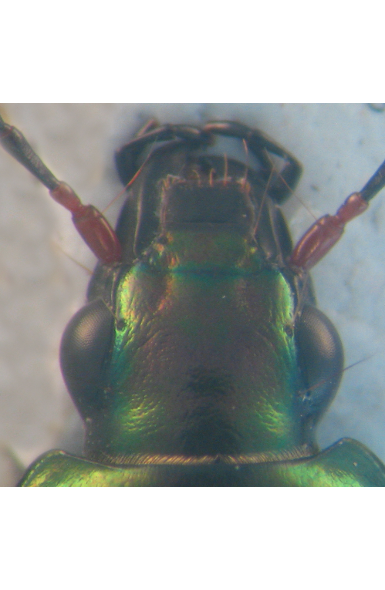
\includegraphics[scale=0.18]{images/tete}}
\Put(-11,-310){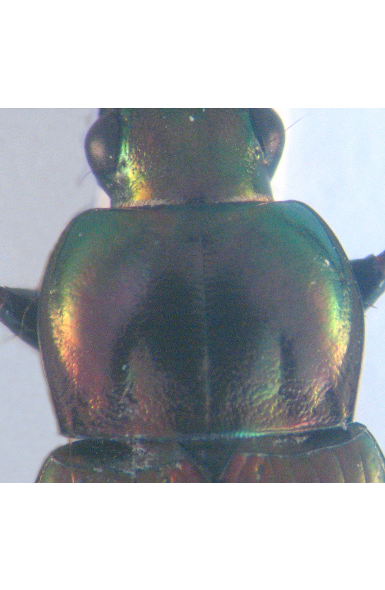
\includegraphics[scale=0.18]{images/pronotum}}
\Put(73,-220){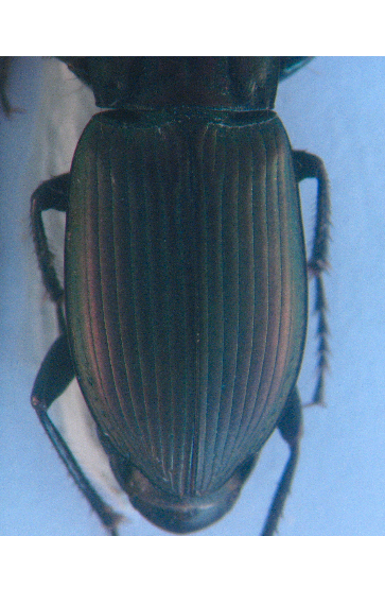
\includegraphics[scale=0.18]{images/elytre}}
\Put(153,-220){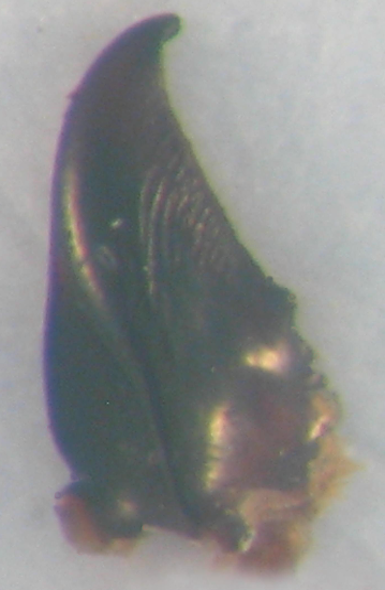
\includegraphics[scale=0.18]{images/mgmo}}
\Put(233,-220){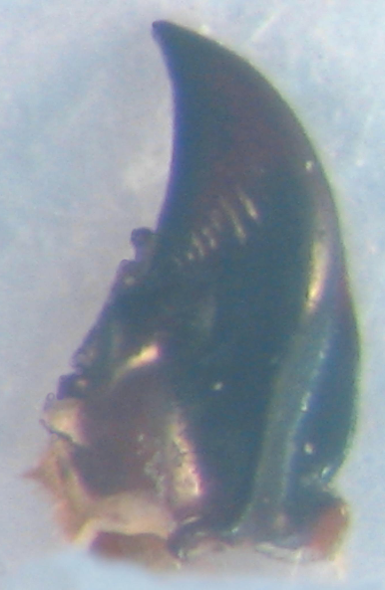
\includegraphics[scale=0.18]{images/mdmo}}
	%\begin{figure}[h]
	%	\centering
	%		\subfloat{\label{figrbox2}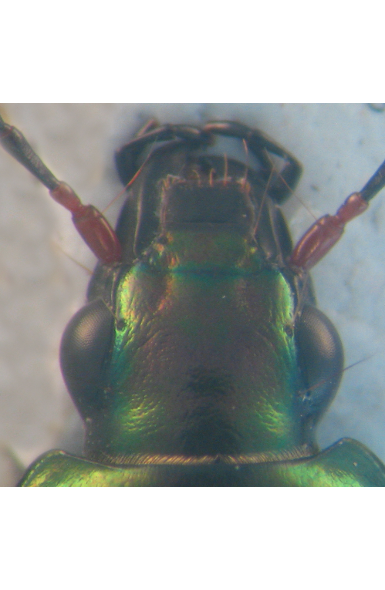
\includegraphics[width=0.2\textwidth]{./images/tete}}~
	%		\subfloat{\label{figrbox2}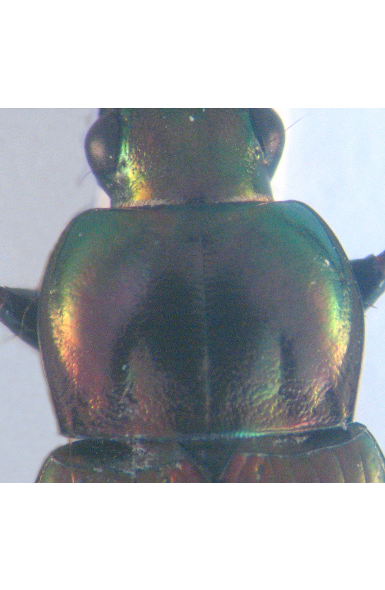
\includegraphics[width=0.2\textwidth]{./images/pronotum}}\\
	%		\subfloat{\label{figrbox2}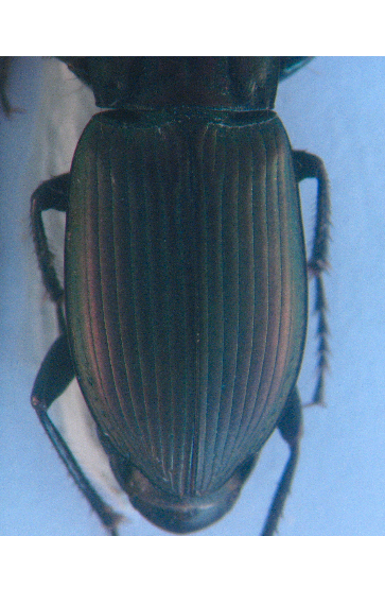
\includegraphics[width=0.2\textwidth]{./images/elytre}}~
	%		\subfloat{\label{figrbox2}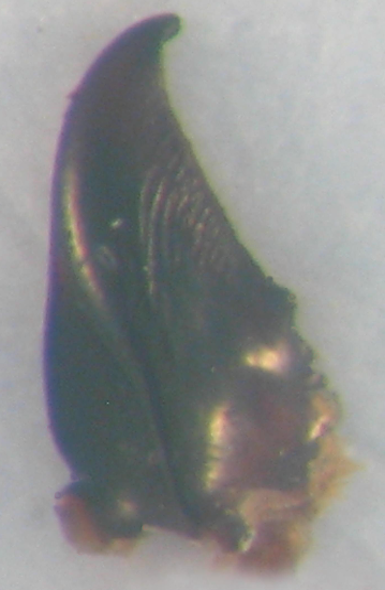
\includegraphics[width=0.2\textwidth]{./images/mgmo}}~
	%		\subfloat{\label{figrbox1}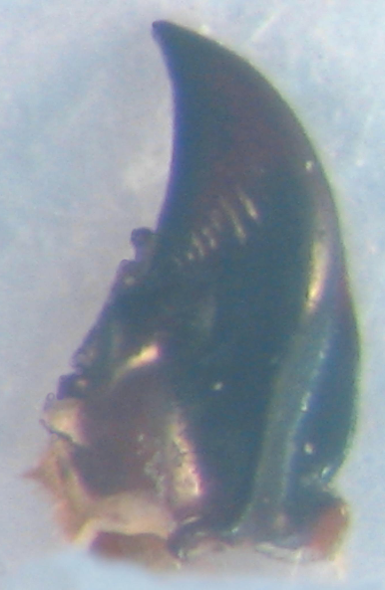
\includegraphics[width=0.2\textwidth]{./images/mdmo}}		
	%\end{figure}
	
	}
	\only<2>{
	\begin{center}
				How to locate automatically the landmarks?
	\end{center}
	\begin{figure}[h]
		\centering
			\subfloat{\label{figrbox2}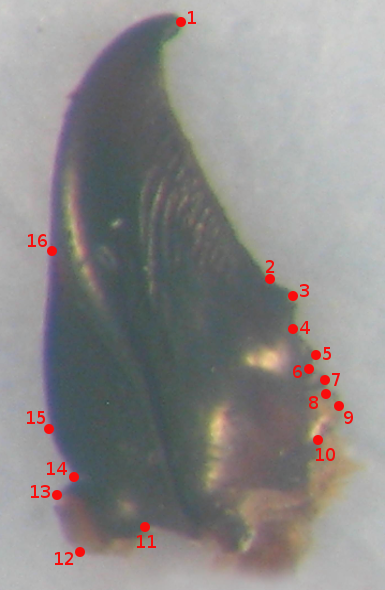
\includegraphics[width=0.35\textwidth]{./images/mgm}}~~
			\subfloat{\label{figrbox1}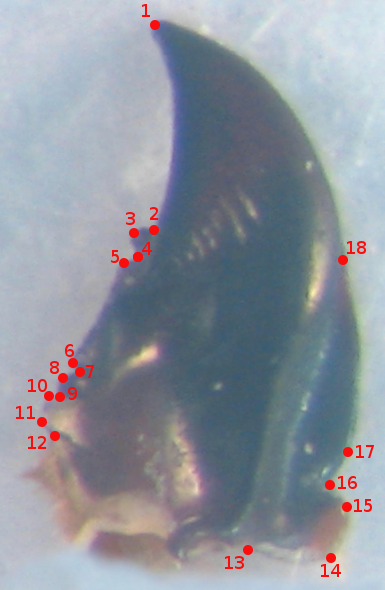
\includegraphics[width=0.35\textwidth]{./images/mdm}}
			%\caption*{Mandibles with manual landmarks (red points)}
\label{fig01s}
\end{figure}
}
\end{frame}
}
{
\setbeamertemplate{headline}{}
\addtobeamertemplate{frametitle}{\vspace*{-0.9\baselineskip}}{}
\begin{frame}
\frametitle{Plan} % Table of contents slide, comment this block out to remove it
\tableofcontents % Throughout your presentation, if you choose to use \section{} and \subsection{} commands, these will automatically be printed on this slide as an overview of your presentation
\end{frame}
}
%----------------------------------------------------------------------------------------
%	PRESENTATION SLIDES
%----------------------------------------------------------------------------------------

%------------------------------------------------
\section[Introduction]{Introduction: {\normalsize overview about the method}}
\subsection*{Overview about the method}
%------------------------------------------------
\begin{frame}
\frametitle{Overview about the method}
\begin{figure}[htb]
    \centering
    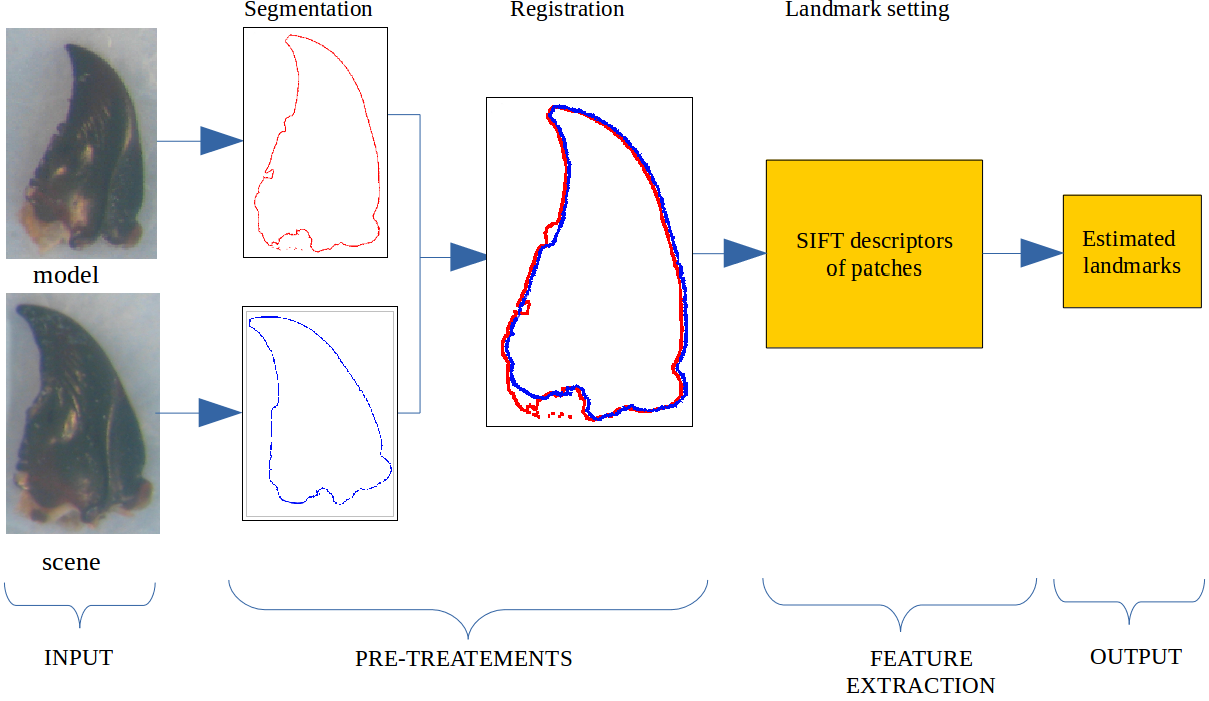
\includegraphics[width=1\textwidth]{./images/method2}
    %\caption{Overview of the proposed method}
    \label{fig2}
\end{figure}
%\begin{block}{}
%\textbf{Input}: two images (model and scene) and model's manual landmarks.\\
%\textbf{Output}: landmarks of the scene image.
%\end{block}
\end{frame}
%------------------------------------------------
\section[Method]{Method: {\normalsize segmentation, registration, SIFT descriptor of patches}}
\subsection*{Method steps in detail}
%------------------------------------------------
\begin{frame}[c]
\frametitle{Segmentation}
	\begin{block}{Algorithm}
		\begin{itemize}[nosep,label=\footnotesize$\bullet$]
			\item Contours as list of points: Canny algorithm\footnotemark.
			\item Threshold ratio: $T_{lower} = (1/3) \times T_{upper}$.
			\item Threshold value ($T_{lower}$): determined by analysing histogram.
		\end{itemize}
	\end{block}
	\pause
	\begin{block}{Result}
		\begin{figure}[h]
		\centering
			\subfloat	{\label{figrbox2}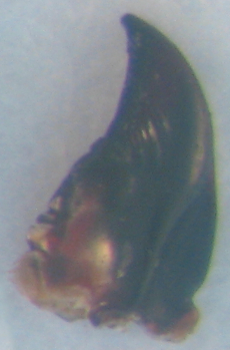
\includegraphics[width=0.2\textwidth]{./images/md}}~~
			\subfloat{\label{figrbox1}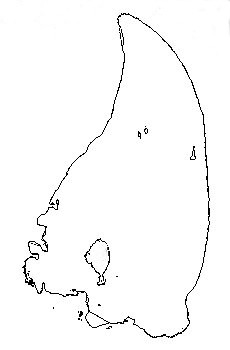
\includegraphics[width=0.2\textwidth]{./images/cannybg}}~~
			\subfloat{\label{figrbox1}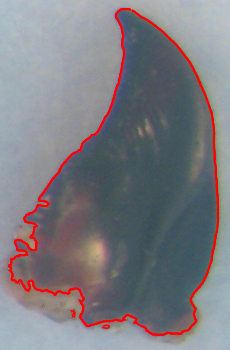
\includegraphics[width=0.2\textwidth]{./images/mdseg}}
			%\caption{Example of a right mandible and its contour points}
%\label{fig1}
\end{figure}
	\end{block}
\footnotetext[1]{{\scriptsize John Canny, \emph{A computational approach to edge detection}, Pattern Analysis and Machine Intelligence, IEEE Transactions on (6):679–698, 1986.}}
\end{frame}
%------------------------------------------------
\begin{frame}{Registration}
%\frametitle{Registration}
\begin{columns}[t] % The "c" option specifies centered vertical alignment while the "t" option is used for top vertical alignment
\column{.5\textwidth} % Left column and width
\begin{block}{PCA Iteration}
\begin{figure}[htb]
    \centering
    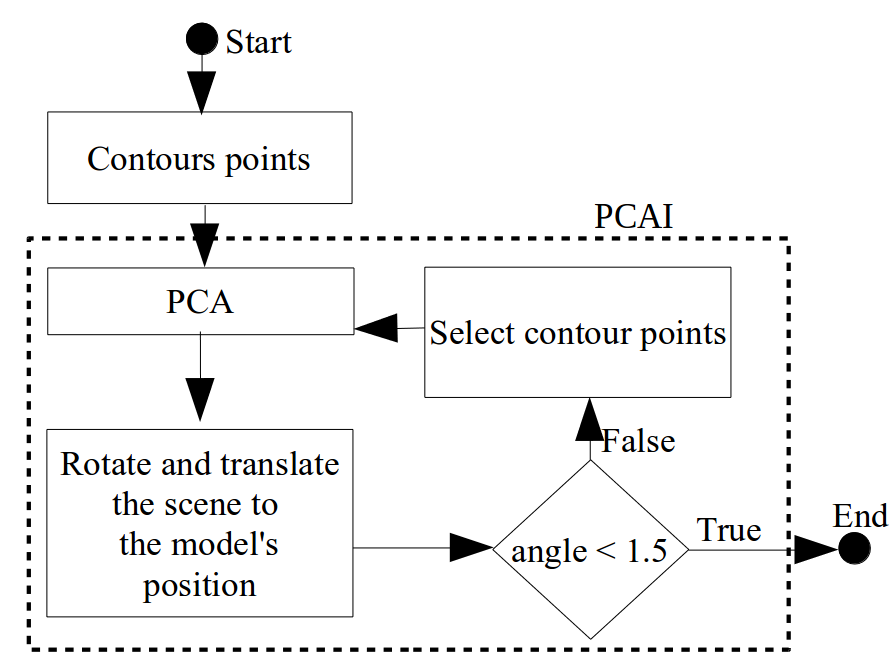
\includegraphics[width=0.95\textwidth]{./images/pcaiill}
    %\caption{Illustration of PCA Iteration.}
    \label{fig3}
\end{figure}
\end{block}
\pause
\column{.5\textwidth} % Right column and width
\begin{block}{Result}
	\begin{figure}[htb]
    \centering
    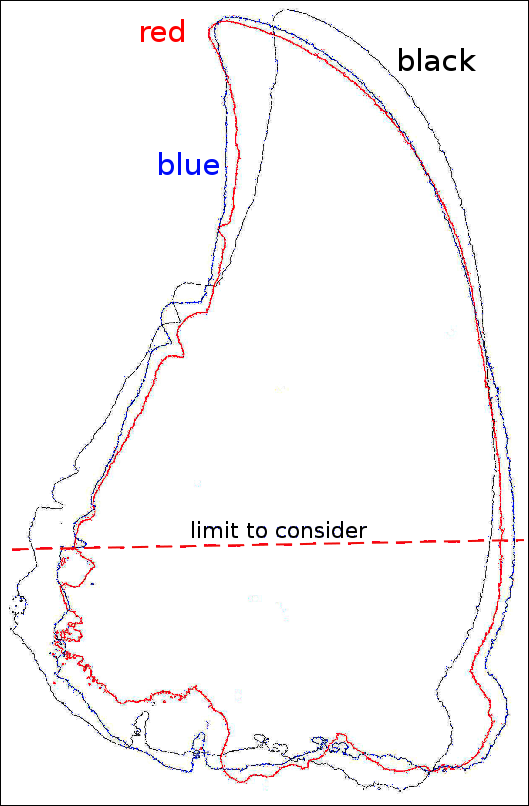
\includegraphics[width=0.75\textwidth]{./images/imreg}
    %\caption{Illustration of PCA Iteration.}
    \label{fig3}
\end{figure}
\end{block}
\end{columns}
\end{frame}
%\begin{frame}
%\frametitle{Method}
%\begin{figure}[htb]
%    \centering
%    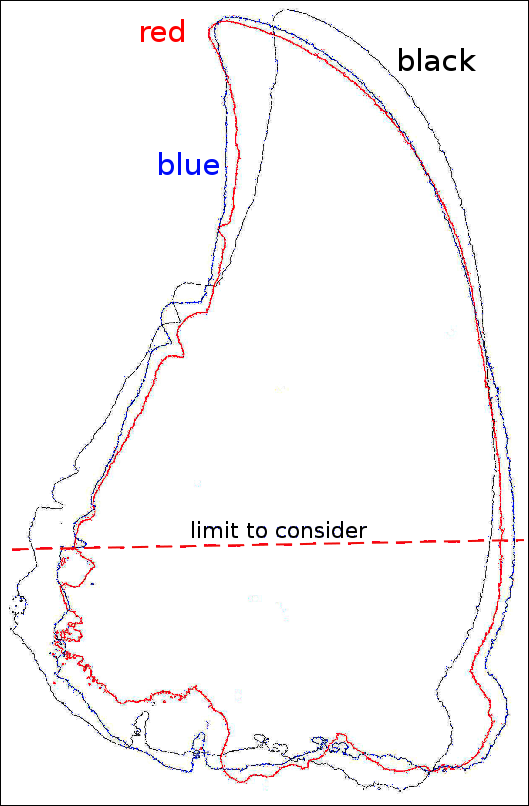
\includegraphics[width=0.35\textwidth]{./images/imreg}
%    \caption{Illustration of PCA Iterations.}
%    \label{fig3}
%\end{figure}
%\end{frame}
\begin{frame}{Landmark setting}
	\begin{columns}[t]
		\column{.6\textwidth}
			\begin{block}{SIFT descriptor}
		\begin{itemize}[nosep,label=\footnotesize$\bullet$]
			\item Proposed by David G Lowe\footnotemark.
			\item \textcolor{red}{Detect} and \textcolor{red}{describe} local features in images.
			\item Many applications: object recognition, robotic mapping, points of interest,...
		\end{itemize}
		\end{block}
		\column{.45\textwidth}
		\begin{block}{SIFT}
		\begin{figure}[htb]
    		\centering
    		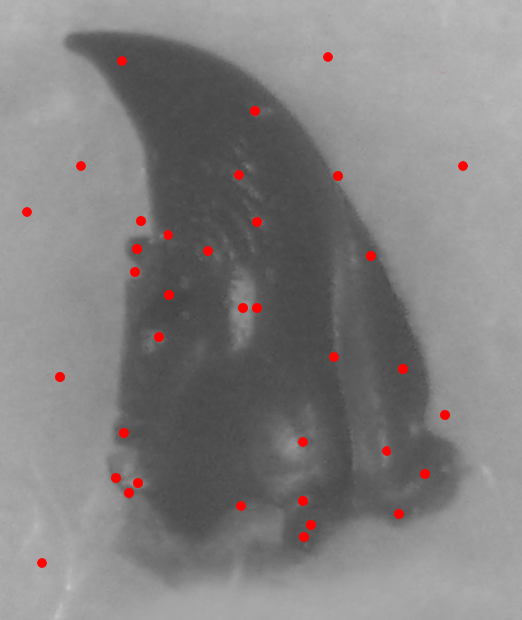
\includegraphics[width=.85\textwidth]{./images/siftc}
		\end{figure}
		\end{block}
		
	
	\end{columns}
	\footnotetext[2]{\scriptsize David G Lowe, \emph{Distinctive image features from scale-invariant keypoints}, International journal of computer vision 60(2):91–110, 2004}
\end{frame}
\begin{frame}{Landmark setting}
	\begin{columns}[t] % The "c" option specifies centered vertical alignment while the "t" option is used for top vertical alignment

\column{.5\textwidth} % Right column and width
\begin{block}{Define the features of landmark}
{\footnotesize 
	\begin{itemize}[leftmargin=*]
		\item Define:
			\begin{itemize}[nosep,label=\footnotesize$\bullet$]
				\item A patch $P_m$ for each model's landmark.
				\item A patch $P_s$ at the same position.
				\item A patch $P'_s$ for every pixels in $P_s$.
			\end{itemize}
		\item Compute:
			\begin{itemize}[nosep,label=\footnotesize$\bullet$]
				\item SIFT descriptor for $P_m$.
				\item SIFT descriptor for $P'_s$.
				\item Compute distance $L(P_m,P'_s)$.
			\end{itemize}
		\item \textcolor{red}{Keep} the pixel that has the \textcolor{red}{minimum} distance.
	\end{itemize}
}
\end{block}
\column{.5\textwidth} % Left column and width
\begin{block}{Illustration}
\begin{figure}[htb]
    \centering
    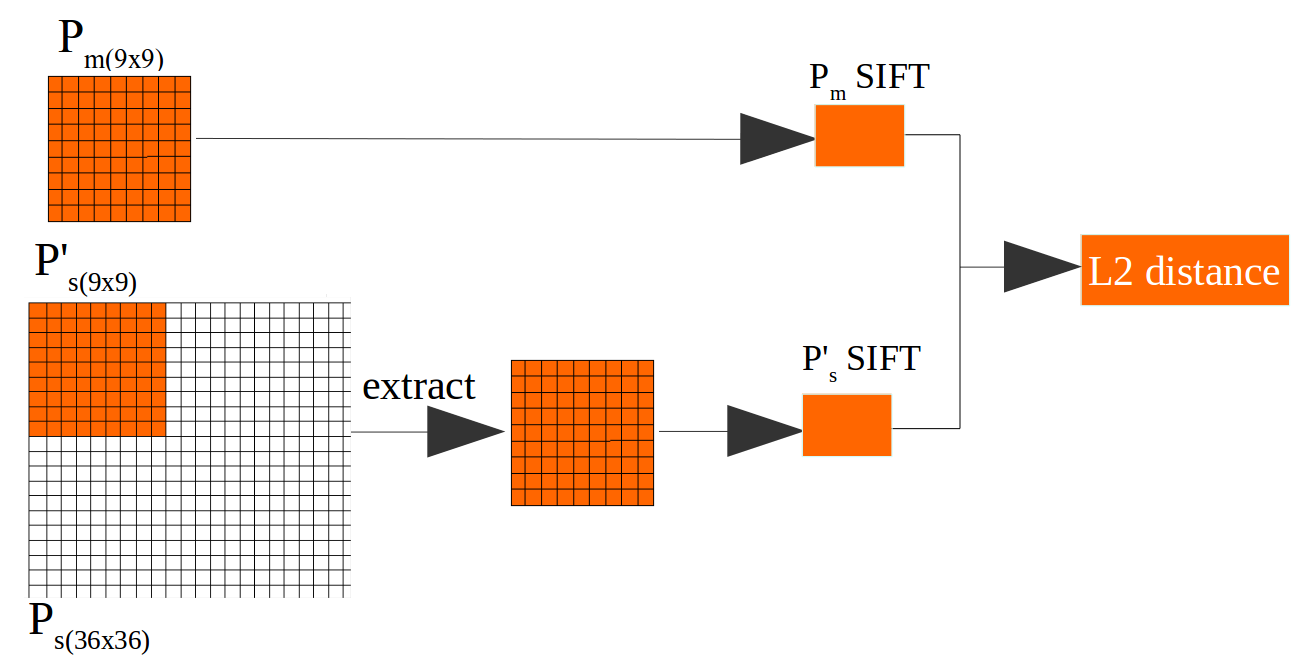
\includegraphics[width=1.0\textwidth]{./images/siftpc}
    \caption*{{\small Illustration of SIFT computing.}}
    \label{fig3}
\end{figure}
\end{block}
{\small
\begin{block}{MAELab}
	\begin{itemize}[nosep,label=\footnotesize$\bullet$]
		\item Library\footnotemark.
		\item Graphic user interface.
	\end{itemize}
\end{block}
}
\end{columns}

\footnotetext[3]{\tiny https://github.com/linhlevandlu/MAELab.git}
\end{frame}
%\begin{frame}
%\frametitle{Method}
%\begin{block}{Landmark estimation}
%How to estimate a landmark on the scene image ?
%	\begin{itemize}
%		\item A region around each model's landmark is computed (called $P_m$),
%		\item Extract in the scene image at the same position (called $P_s$)
%		\item Calculate the SIFT descriptor for $P_m$
%		\item For each pixel in $P_s$, extract a patch $P'_s$ with the same size than $P_m$.
%		\item Compute the SIFT descriptor for $P'_s$
%		\item Compute the distance $L(P_m, P'_s)$.
%		\item Keep the pixel in $P_s$ that has the minimum distance.
%	\end{itemize}
%\end{block}
%\end{frame}

%\begin{frame}
%\frametitle{Method}
%\begin{block}{Landmark estimation}
%	\begin{figure}[htb]
%    \centering
%    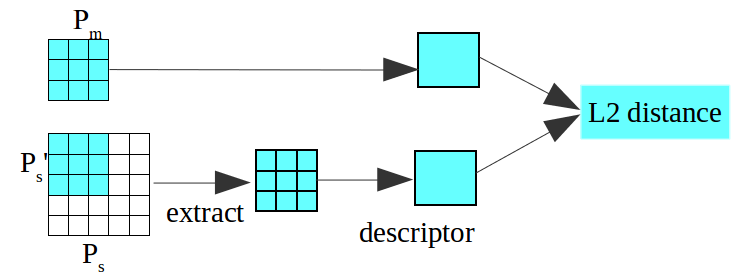
\includegraphics[width=0.70\textwidth]{./images/illustration_SIFT}
%    \caption{Steps of SIFT descriptors comparison.}
%    \label{fig3}
%\end{figure}
%\end{block}
%\end{frame}

%------------------------------------------------
\section[Result]{Result: {\normalsize final result and evaluation}}
\subsection*{Result}
%------------------------------------------------

\begin{frame}[t]
\frametitle{Landmarks position}
%\def\Put(#1,#2)#3{\leavevmode\makebox(0,0){\put(#1,#2){#3}}}
\Put(-20,-100){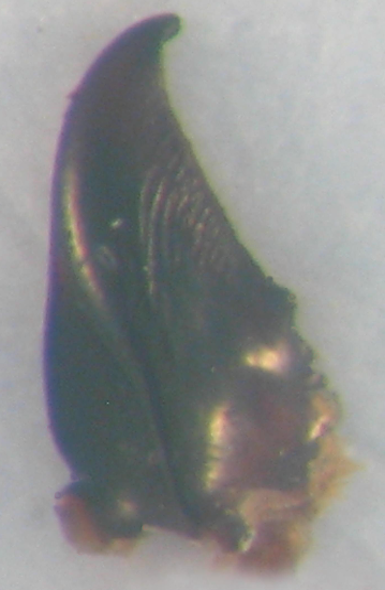
\includegraphics[scale=0.11]{images/mgmo.png}}
\Put(-15,-120){{\small model}}
\Put(280,-100){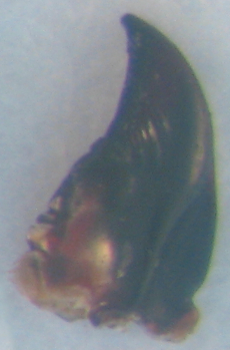
\includegraphics[scale=0.18]{images/md.png}}
\Put(285,-120){{\small model}}
\Put(20,-305){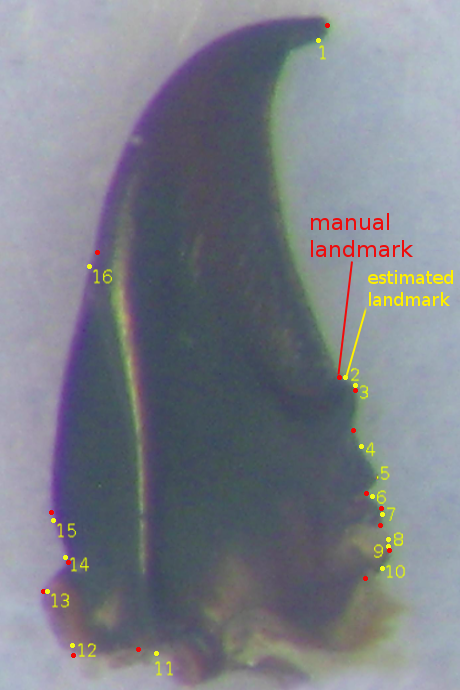
\includegraphics[width=0.37\textwidth]{./images/mg_rs2}}
\Put(50,-330){{\small scene }}
\Put(140,-305){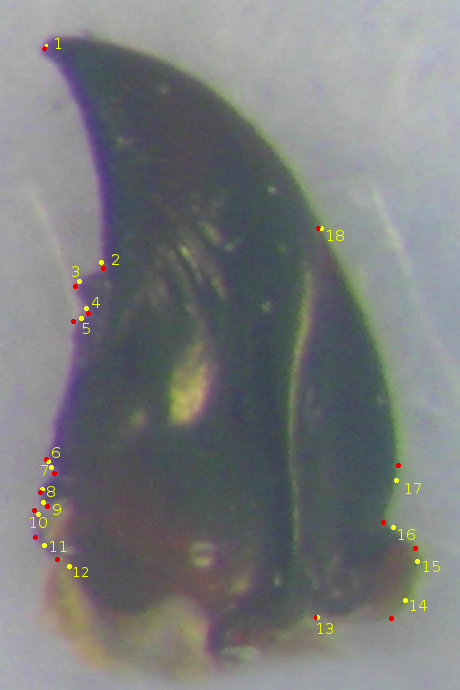
\includegraphics[width=0.37\textwidth]{./images/md_rs}}
\Put(160,-330){{\small scene }}
%\begin{figure}[h]
%		\centering
%			\subfloat[{\footnotesize A left mandible}]				{\label{figrbox2}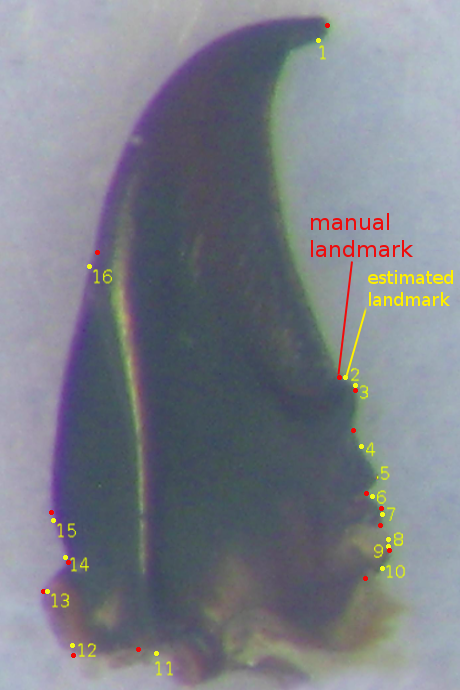
\includegraphics[width=0.35\textwidth]{./images/mg_rs2}}~~
%			\subfloat[{\footnotesize A right mandible}]{\label{figrbox1}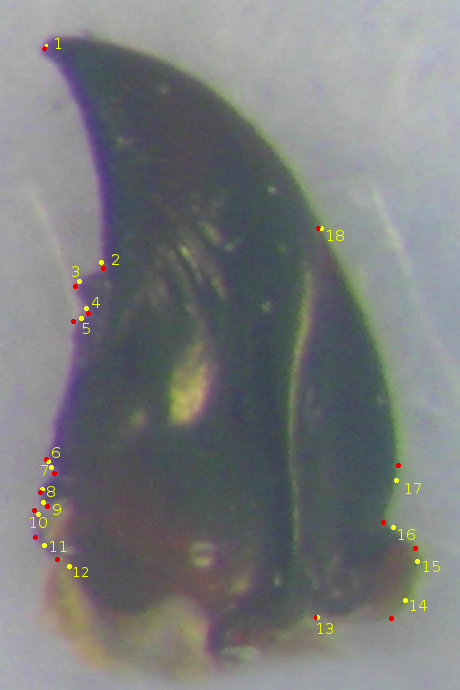
\includegraphics[width=0.35\textwidth]{./images/md_rs}}
%			\caption*{\footnotesize The mandibles with the manual (red) and estimated (yellow) landmarks}
%\label{fig1}
%\end{figure}
\Put(0,-360){\textbf{Red}: manual landmarks. \textbf{Yellow}: estimated landmarks}
\end{frame}

%------------------------------------------------
%------------------------------------------------
\begin{frame}
\frametitle{Evaluation}
	\begin{block}{Statistic}
	\begin{itemize}[nosep,label=\footnotesize$\bullet$]
		\item Calculate the distance between the estimated landmark $p$ and corresponding manual landmark $q$\\.
		\begin{center}
			$d(p,q) = \sqrt{(p_x - q_x)^2 + (p_y - q_y)^2}$
		\end{center}
		\item The statistic is done on all images with a standard deviation error.
	\end{itemize}
	\end{block}
\end{frame}
\begin{frame}
\frametitle{Statistic on right mandible}
\begin{columns}[t]
\column{.7\textwidth}
{\small
\begin{block}{Summary}
\begin{itemize}[nosep,label=\footnotesize$\bullet$]
	\item Highest accuracy: \textbf{$1^{st}$} landmark with 98.62\%.
	\item Lowest accuracy: \textbf{$13^{th}, 14^{th}$} landmark with app. 75\%.
\end{itemize}
\end{block}
}
\Put(15,-200){    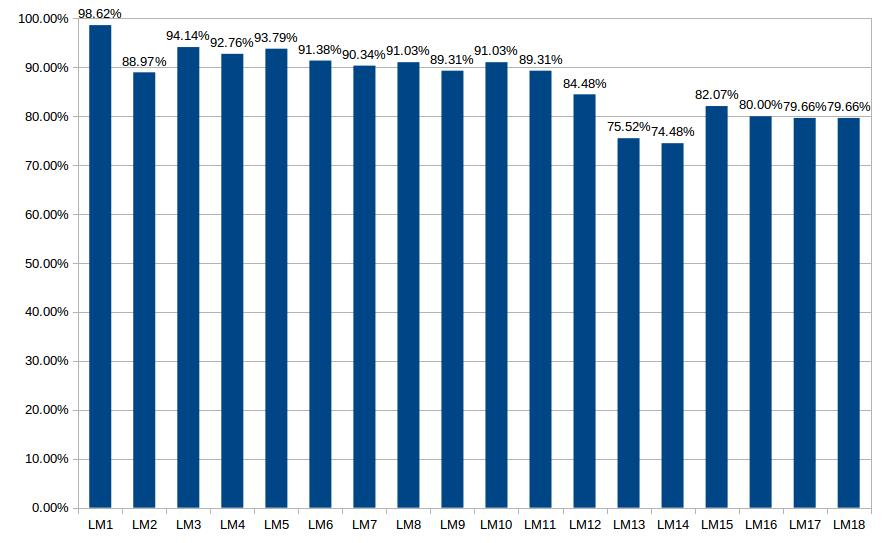
\includegraphics[width=0.85\textwidth]{./images/md_chartlms}}
%\begin{figure}[htb]
%    \centering
%    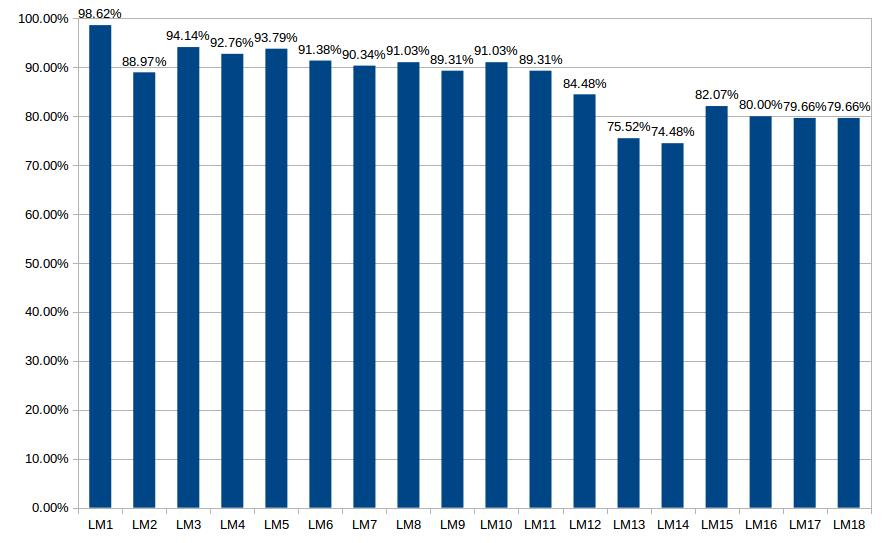
\includegraphics[scale=.25]{./images/md_chartlms}
%    \label{fig3}
%\end{figure}
\column{.3\textwidth}
\begin{figure}[htb]
    \centering
    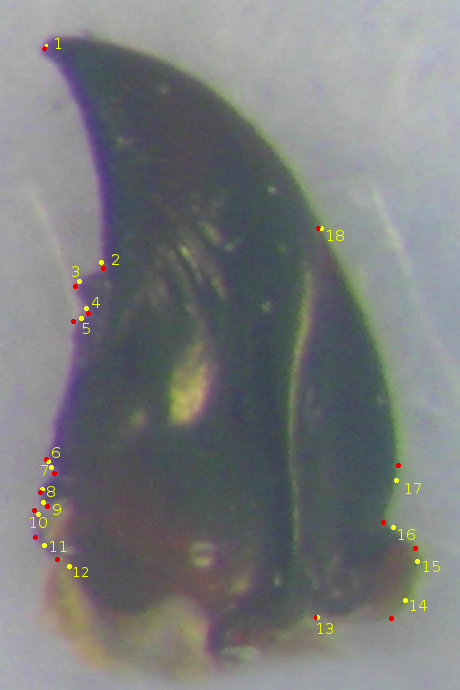
\includegraphics[width=1\textwidth]{./images/md_rs}
    %\caption{The proportions of well estimated landmark of right mandibles.}
\end{figure}
\end{columns}
\end{frame}

\begin{frame}
\frametitle{Statistic on left mandible}
\begin{columns}[t]
\column{.7\textwidth}
\begin{block}{Summary}
{\small
\begin{itemize}[nosep,label=\footnotesize$\bullet$]
	\item Highest accuracy: \textbf{$1^{st}$} landmark with 93.01\%.
	\item Lowest accuracy: \textbf{$11^{th}, 12^{th} \text{ } and \text{ } 16^{th}$} landmark with 60.14\%.
\end{itemize}
}
\end{block}
\begin{figure}[htb]
    \centering
    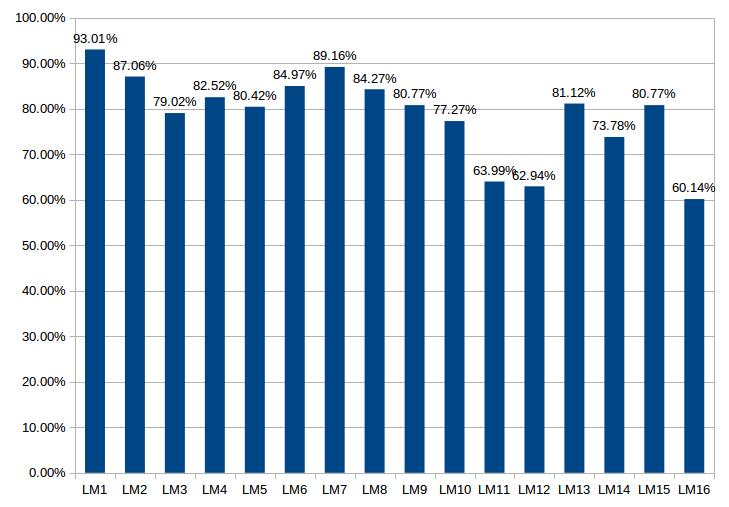
\includegraphics[width=0.8\textwidth]{./images/mg_chartlms}
 %   \caption*{The proportions of well estimated landmark of left mandibles.}
    \label{fig3}
\end{figure}
\column{.3\textwidth}
\begin{figure}[htb]
    \centering
    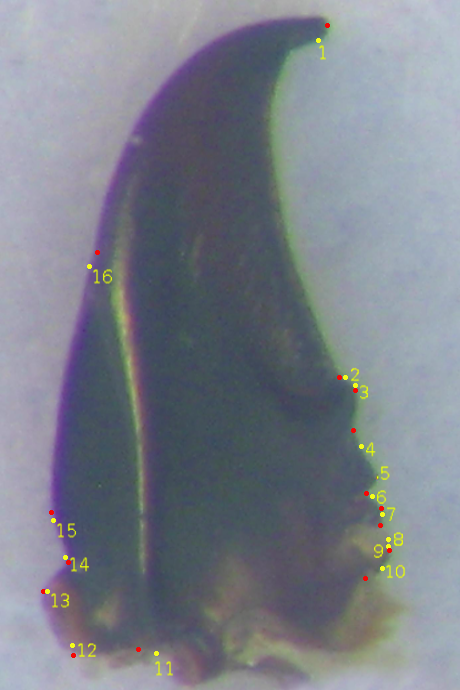
\includegraphics[width=0.97\textwidth]{./images/mg_rs}
\end{figure}
\end{columns}
\end{frame}

%------------------------------------------------
\section{Conclusion and future works}
\subsection*{Conclusion}
\begin{frame}
\frametitle{Conclusion}
	\
	\begin{itemize}[nosep,label=\footnotesize$\bullet$]
		\item Proposed method to \textcolor{red}{determine landmarks automatically} on beetle mandibles including: segmentation, registration and estimation.
		\item The location of the estimated landmarks are \textcolor{red}{workable} with high proportion.
		\item Perspective, when considering the \textcolor{red}{centroid} of the object, the result from method is very good.
		\item Method is useful for biologist. It solves the \textcolor{red}{time-consuming} problem during setting the landmarks.
	\end{itemize}
	
\end{frame}
%----------------------------------------------------
%----------------------------------------------------
\begin{frame}
\frametitle{Working with other parts}
 \begin{figure}[htb]
    \centering
    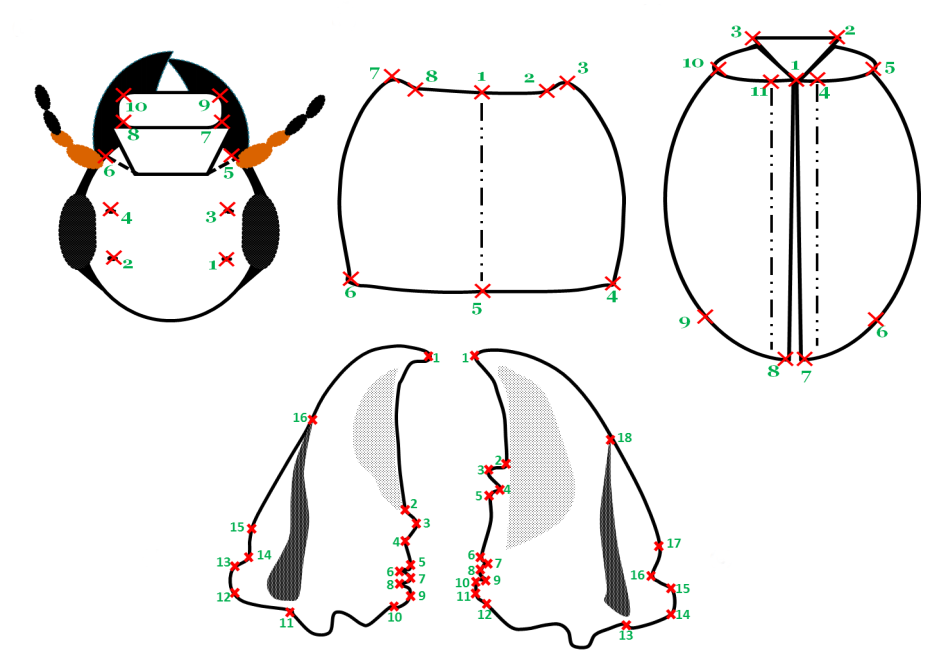
\includegraphics[width=0.95\textwidth]{./images/conclusion}
    %\caption{Overview of the proposed method}
    \label{fig2}
\end{figure}
\end{frame}
%\begin{frame}
%\frametitle{Future works}
%\begin{itemize}[nosep,label=\footnotesize$\bullet$]
%		\item Working with other parts of beetle,
%		\item Applying deep learning (Convolutional Neural Network) to detect the landmarks,
%		\item Integrating our work with automatic classification.
%	\end{itemize}
%\end{frame}
%------------------------------------------------
\begin{frame}
\Huge{\centerline{Thank you}}
\end{frame}
%------------------------------------------------

\begin{frame}
\frametitle{References}
\footnotesize{
\begin{thebibliography}{99} % Beamer does not support BibTeX so references must be inserted manually as below
\bibitem[bec03]{p1} José Maria Becerra and Antonio G Valdecasas
\newblock Landmark superimposition for taxonomic identification
\newblock \emph{Biological Journal of the Linnean Society} 81:page 267–274, 2004.

\bibitem[bland1996statistics]{p2} J Martin Bland and Douglas G Altman
\newblock Statistics notes: measurement error
\newblock \emph{Bmj} 313(7059):744, 1996.

\bibitem[paul2014]{p1} Paul A Bromiley, Anja C Schunke, Hossein
Ragheb, Neil A Thacker, and Diethard Tautz
\newblock Semi-automatic landmark point annotation for geometric morphometrics
\newblock \emph{Frontiers in Zoology} 11(1):61, 2014.

\bibitem[Le2016]{p1} L Lê Vãnh, M Beurton-Aimar, JP Salmon,
A Marie, and N Parisey
\newblock Estimating landmarks on 2d images of beetle mandibles
\newblock \emph{WSCG} 2016.

\bibitem[canny1986]{p1} John Canny
\newblock A computational approach to edge detection
\newblock \emph{Pattern Analysis and Machine Intelligence, IEEE Transactions on} (6):679–698, 1986.
\end{thebibliography}
}
\end{frame}

\begin{frame}
\frametitle{References}
\footnotesize{
\begin{thebibliography}{99} % Beamer does not support BibTeX so references must be inserted manually as below
\bibitem[leila2010]{p1} Leila Favaedi and Maria Petrou
\newblock Cephalometric landmarks identification using probabilistic
relaxation
\newblock \emph{Engineering in Medicine and Biology Society (EMBC), 2010 Annual International Conference of the IEEE} pages 4391 – 4394. IEEE,
2010.

\bibitem[houle2003]{p2} David Houle, Jason Mezey, Paul Galpern, and Ashley Carter
\newblock Automated measurement of drosophila wings
\newblock \emph{BMC evolutionary biology} 3(1):25, 2003.

\bibitem[dehua2011]{p1} Dehua Li Jun Zeng
\newblock An adaptive canny edge detector using histogram concavity analysis
\newblock \emph{International Journal of Digital Content Technology
and its Applications} 5, 2011.

\bibitem[yanke2004]{p1} Yan Ke and Rahul Sukthankar
\newblock Pca-sift: A more distinctive representation for local image descriptors
\newblock \emph{CVPR 2004. Proceedings of the 2004
IEEE Computer Society Conference on} volume 2,
pages II–II. IEEE, 2004.

\bibitem[li2009]{p1} Yunpeng Li, David. J Crandall, and Daniel P.
Huttenlocher
\newblock Landmark classification in large scale image collections
\newblock \emph{Computer vision, 2009 IEEE 12th international conference on                                                                                                 } pages 1957–1964. Kyoto, Japan, 29 sept-2 oct 2009.
\end{thebibliography}
}
\end{frame}

\begin{frame}
\frametitle{References}
\footnotesize{
\begin{thebibliography}{99} % Beamer does not support BibTeX so references must be inserted manually as below
\bibitem[lowe2004]{p1} David G Lowe
\newblock Distinctive image features from scale-invariant keypoints
\newblock \emph{International journal of computer vision} 60(2):91–110, 2004

\bibitem[palaniswamy2010]{p2} Sasirekha Palaniswamy, Neil A Thacker, and Christian Peter Klingenberg
\newblock Automatic identification of landmarks in digital images
\newblock \emph{IET Computer Vision} 4(4):247–260, 2010.

\bibitem[pearson1901]{p1} K. Pearson
\newblock On lines and planes of closest fit to systems of points in space
\newblock \emph{Philosophical Magazine} 2(6):559–572, 1901.

\bibitem[shlens2014]{p1} Jonathon Shlens
\newblock A tutorial on principal component analysis
\newblock \emph{} 1404.1100, 2014.

\bibitem[zhang2014]{p1} Zhanpeng Zhang, Ping Luo, Chen Change Loy,
and Xiaoou Tang
\newblock Facial landmark detection by deep multi-task learning
\newblock \emph{European Conference
on Computer Vision} pages 94–108. Springer, 2014.
\end{thebibliography}
}
\end{frame}

%------------------------------------------------

%----------------------------------------------------------------------------------------

\end{document} 
